\section{Auswertung}

\subsection{Bestimmung der Strömungsgeschwindigkeit}

In Tabelle \ref{tab:stroemi} sind alle Messwerte des ersten Versuchsteils zu finden. Dabei werden die Strömungsgeschwindigkeiten mithilfe von Gleichung \ref{eq:eq4}, die nach $v$ umgestellt wird, berechnet. 

\begin{equation}
v = \frac{\Delta \nu \cdot c}{2\nu_0\cdot cos(\alpha)}.
\label{eq:eq6}
\end{equation}

Die Schallgeschwindigkeit in der Dopplerflüssigkeit beträgt $c = 1800\,\symup{\frac{m}{s}}$ und die Frequenz der Ultraschallwelle ist $\nu_0 = 2 \cdot 10^{6}\,\symup{Hz}$ \cite[3, 4]{anleitungUS3}. Die Dopplerwinkel der jeweiligen Prismenwinkel werden über
Gleichung \ref{eq:eq7} bestimmt. Zu finden sind diese in Tabelle \ref{tab:winkel}.

\begin{table}[htbp]
\centering
\caption{Prismen- und Dopplerwinkel.}
\label{tab:winkel}
\begin{tabular}{S[table-format=2] S[table-format=2.2]}
\toprule
{$\theta/ \,°$} & {$\alpha/\,°$} \\
\midrule
15 & 80.06\\
30 & 70.53\\
60 & 54.74\\
\bottomrule
\end{tabular}
\end{table}

Aus den im Versuch gemessenen Werten werden die jeweiligen Strömungsgeschwindigkeiten $v$ berechnet, sowie die Quotienten $\frac{\lvert \Delta \nu \rvert}{cos(\alpha)}$. Alle Messergebnisse sind in Tabelle \ref{tab:stroemi} zu finden.
In Abbildung \ref{fig:stroemi} ist für die drei Dopplerwinkel $\frac{\lvert \Delta \nu \rvert}{cos(\alpha)}$ gegen die Strömungsgeschwindigkeit $v$ aufgetragen.


\begin{table}[htbp]
\centering
\caption{Messwerte zur Untersuchung der Strömungsgeschwindigkeit $v$.}
\label{tab:stroemi}
\begin{tabular}{S[table-format=1.1] S[table-format=2] S S[table-format=4] S[table-format=1.4] S[table-format=4.2]}
\toprule
{$\dot{V}/ \, \symup{\frac{l}{min}}$} & {$d/10^{-3}\, \symup{m}$} & {$\alpha/ \, °$} & {$\lvert \Delta \nu \rvert / \, \symup{Hz}$} & {$v /\,\symup{\frac{m}{s}}$} & {$\frac{\lvert \Delta \nu \rvert}{cos(\alpha)} /\,\symup{Hz}$}  \\
\midrule
        &       & 15 & 537 & 1.39 & 3110.94\\
        & 10    & 30 & 665 & 0.89 & 1995.12\\
        &       & 60 & 1282 & 0.99 & 2220.73\\
\cmidrule{2-6}	
        &       & 15 & 159 & 0.41 & 921.12\\
2.8     & 15    & 30 & 256 & 0.35 & 768.05\\
        &       & 60 & 415 & 0.32 & 718.88\\
\cmidrule{2-6}
        &       & 15 & 98 & 0.26 & 567.73\\
        & 20    & 30 & 110 & 0.15 & 330.02\\
        &       & 60 & 232 & 0.18 & 401.88\\
\midrule
        &       & 15 & 659 & 1.72 & 3817.71\\
        & 10    & 30 & 1013 & 1.37 & 3039.18\\
        &       & 60 & 1508 & 1.18 & 2612.22\\
\cmidrule{2-6}
        &       & 15 & 159 & 0.41 & 921.12\\
3.3     & 15    & 30 & 342 & 0.46 & 1026.06\\
        &       & 60 & 596 & 0.46 & 1032.41\\
\cmidrule{2-6}
        &       & 15 & 85  & 0.22 & 492.42\\
        & 20    & 30 & 134 & 0.18 & 402.02\\
        &       & 60 & 232 & 0.18 & 401.88\\
\midrule
        &       & 15 & 769 & 2.00 & 4454.95\\
        & 10    & 30 & 1257 & 1.69 & 3771.23\\
        &       & 60 & 1868 & 1.46 & 3235.82\\
\cmidrule{2-6}
        &       & 15 & 208 & 0.54 & 1204.98\\
3.7     & 15    & 30 & 391 & 0.53 & 1173.07\\
        &       & 60 & 751 & 0.26 & 1300.91\\
\cmidrule{2-6}
        &       & 15 & 85 & 0.22 & 492.42\\
        & 20    & 30 & 171 & 0.23 & 513.03\\
        &       & 60 & 1160 & 0.40 & 2009.39\\
\midrule
        &       & 15 & 928 & 2.42 & 5376.07\\
        & 10    & 30 & 1447 & 1.95 & 4341.26\\
        &       & 60 & 2063 & 0.71 & 3573.61\\
\cmidrule{2-6}
        &       & 15 & 220 & 0.57 & 1274.49\\
4.2     & 15    & 30 & 452 & 0.61 & 1356.08\\
        &       & 60 & 812 & 0.28 & 1406.58\\
\cmidrule{2-6}
        &       & 15 & 110 & 0.29 & 637.25\\
        & 20    & 30 & 201 & 0.27 & 603.04\\
        &       & 60 & 464 & 0.16 & 803.76\\
\midrule
        &       & 15 & 1025 & 2.67 & 5938.01\\
        & 10    & 30 & 1190 & 1.61 & 3570.22\\
        &       & 60 & 2350 & 0.81 & 4070.76\\
\cmidrule{2-6}
        &       & 15 & 256 & 0.67 & 1483.05\\
4.7     & 15    & 30 & 555 & 0.75 & 1665.10\\
        &       & 60 & 1086 & 0.38 & 1881.21\\
\cmidrule{2-6}
        &       & 15 & 122 & 0.32 & 706.77\\
        & 20    & 30 & 269 & 0.36 & 807.05\\
        &       & 60 & 305 & 0.11 & 528.33\\
\bottomrule
\end{tabular}
\end{table}


\begin{figure}[h!tbp]
	\centering
	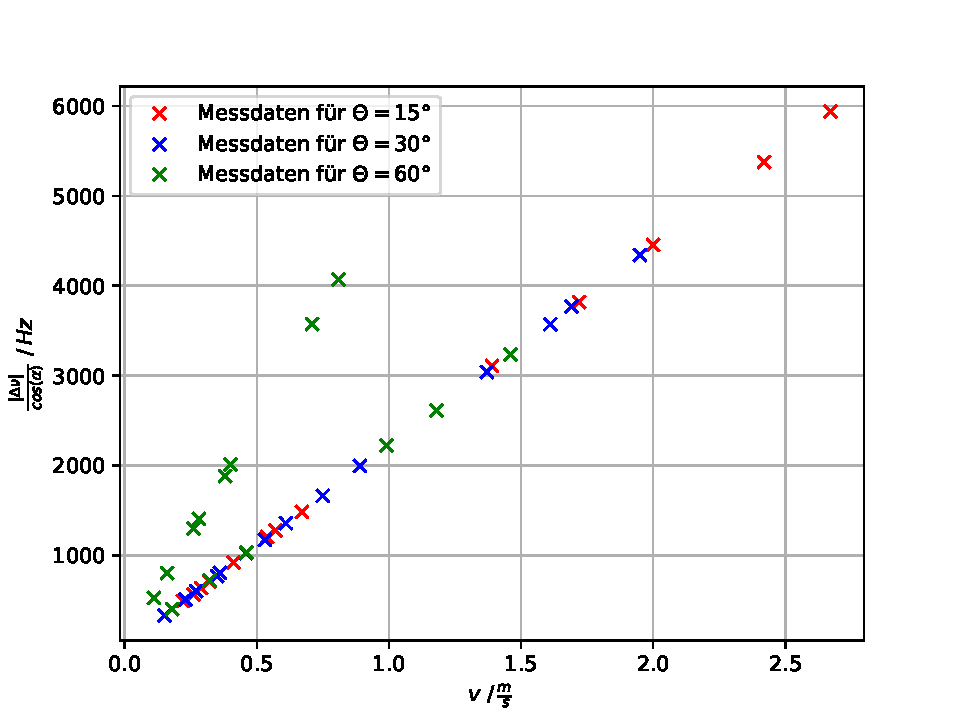
\includegraphics[width=0.8\linewidth]{graph1.pdf}
	\caption{$\frac{\lvert \Delta \nu \rvert}{cos(\alpha)}$ als Funktion der Strömungsgeschwindigkeit $v$.}
	\label{fig:stroemi}
\end{figure}






\newpage
\subsection{Bestimmung des Strömungsprofils}

Zur Bestimmung des Strömungsprofils wird die Messung bei einer Tiefe von $l = 30\cdot10^{-3}\,\symup{m}$ begonnen, wo das Prisma endet und der eigentliche Messbereich anfängt. Umgerechnet wird dies mit $4\,\symup{\mu s} = 10\cdot10^{-3}\,\symup{m}$, 
was also einer Messtiefe von $y = 12\,\symup{\mu s}$ entspricht. In der Dopplerflüssigkeit wird mit $4\,\symup{\mu s} = 6\cdot10^{-3}\,\symup{m}$ umgerechnet.
In Tabelle \ref{tab:profil} sind die Messtiefen $y$, die Eindringtiefen $x$, die gemessenen Frequenzverschiebungen $\Delta \nu$ und die Streuintensitäten $I$, sowie die über Gleichung \ref{eq:eq6} berechneten Strömungsgeschwindigkeiten $v$ zu finden.
In den Abbildungen \ref{fig:profil1} und \ref{fig:profil3} sind die Strömungsgeschwindigkeiten der jeweiligen Volumenströme gegen die Eindringtiefe aufgetragen, in Abbildungen \ref{fig:profil2} und \ref{fig:profil4} sind die Streuintensitäten die Funktion 
der Eindringtiefe.

\begin{table}[htbp]
\centering
\caption{Messwerte zur Untersuchung des Strömungsprofils.}
\label{tab:profil}
\begin{tabular}{S[table-format=2.1] S[table-format=2.2] S[table-format=2.3] S[table-format=2.2] S[table-format=2.3] S[table-format=1.2]  }
\toprule
{$\dot{V}/ \, \symup{\frac{l}{min}}$} & {$y/10^{-6}\, \symup{s}$} &  {$x/10^{-3}\, \symup{m}$} & {$\lvert \Delta \nu \rvert / \, \symup{Hz}$} & {$I/\, \%$} &  {$v /\,\symup{\frac{m}{s}}$}\\
\midrule
       & 12.0 & 0.00   & 220 & 7.1 & 0.57\\
       & 12.5 & 0.75 & 256 & 6.7 & 0.67\\
       & 13.0 & 1.50   & 391 & 4.2 & 1.02\\
       & 13.5 & 2.25 & 488 & 3.2 & 1.27\\
       & 14.0 & 3.00   & 586 & 3.0 & 1.53\\
       & 14.5 & 3.75 & 635 & 3.6 & 1.66\\
       & 15.0 & 4.50   & 635 & 2.8 & 1.66\\
4.8    & 15.5 & 5.25 & 513 & 3.2 & 1.34\\
       & 16.0 & 6.00   & 427 & 3.6 & 1.11\\
       & 16.5 & 6.75 & 287 & 8.2 & 0.75\\
       & 17.0 & 7.50   & 232 & 8.6 & 0.60\\
       & 17.5 & 8.25 & 244 & 14.6 & 0.64\\
       & 18.0 & 9.00  & 366 & 13.0 & 0.95\\
       & 18.5 & 9.75 & 378 & 8.7 & 0.99\\
       & 19.0 & 10.50  & 354 & 10.6 & 0.92\\
       & 19.5 & 11.25 & 317 & 7.4 & 0.83\\
\midrule
       & 12.0 & 0.00    & 159 & 9.6 & 0.41\\
       & 12.5 & 0.75 & 171 & 8.6 & 0.45\\
       & 13.0 & 1.50  & 208 & 6.3 & 0.54\\
       & 13.5 & 2.25 & 281 & 4.8 & 0.73\\
       & 14.0 & 3.00 & 330 & 4.0 & 0.86\\
       & 14.5 & 3.75 & 366 & 4.2 & 0.95\\
       & 15.0 & 4.50 & 366 & 3.4 & 0.95\\
3.4    & 15.5 & 5.25 & 354 & 3.0 & 0.92\\
       & 16.0 & 6.00 & 305 & 3.3 & 0.79\\
       & 16.5 & 6.75 & 232 & 6.1 & 0.60 \\
       & 17.0 & 7.50 & 159 & 10.2 & 0.41\\
       & 17.5 & 8.25 & 134 & 9.5 & 0.35\\
       & 18.0 & 9.00 & 208 & 10.3 & 0.54\\
       & 18.5 & 9.75 & 220 & 11.8 & 0.57\\
       & 19.0 & 10.50 & 220 & 10.9 & 0.57\\
       & 19.5 & 11.25 & 195 & 9.6 & 0.51\\

\bottomrule
\end{tabular}
\end{table}


\begin{figure}[h!tbp]
	\centering
	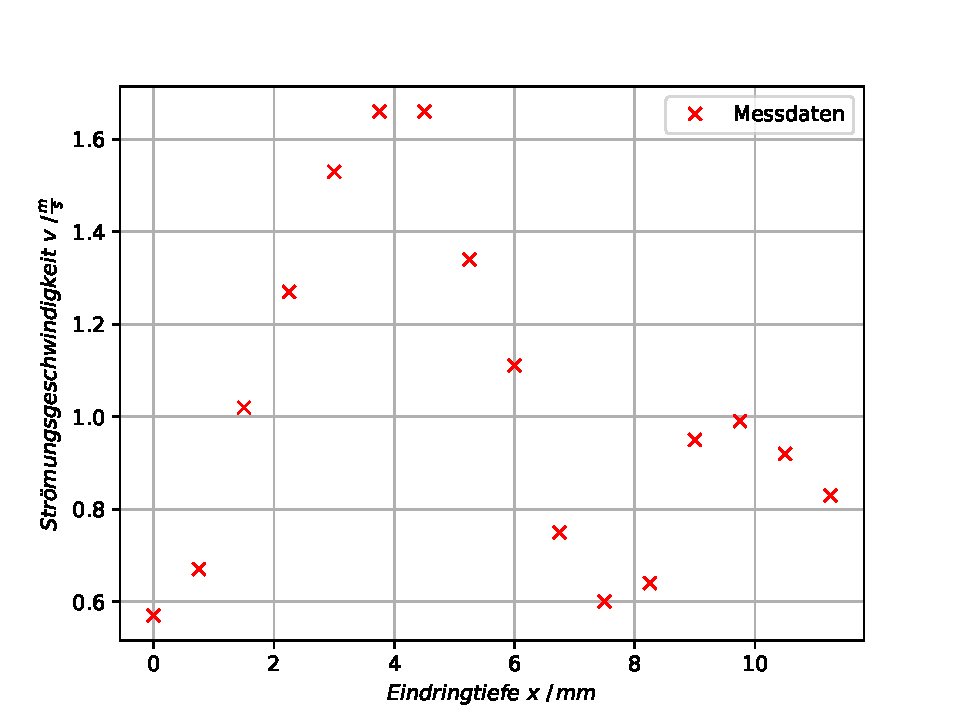
\includegraphics[width=0.8\linewidth]{geschw_48.pdf}
	\caption{Strömungsgeschwindigkeit $v$ als Funktion der Eindringtiefe $x$ bei $\dot{V} = 4{,}8\,\symup{\frac{l}{min}}$.}
	\label{fig:profil1}
\end{figure}


\begin{figure}[h!tbp]
	\centering
	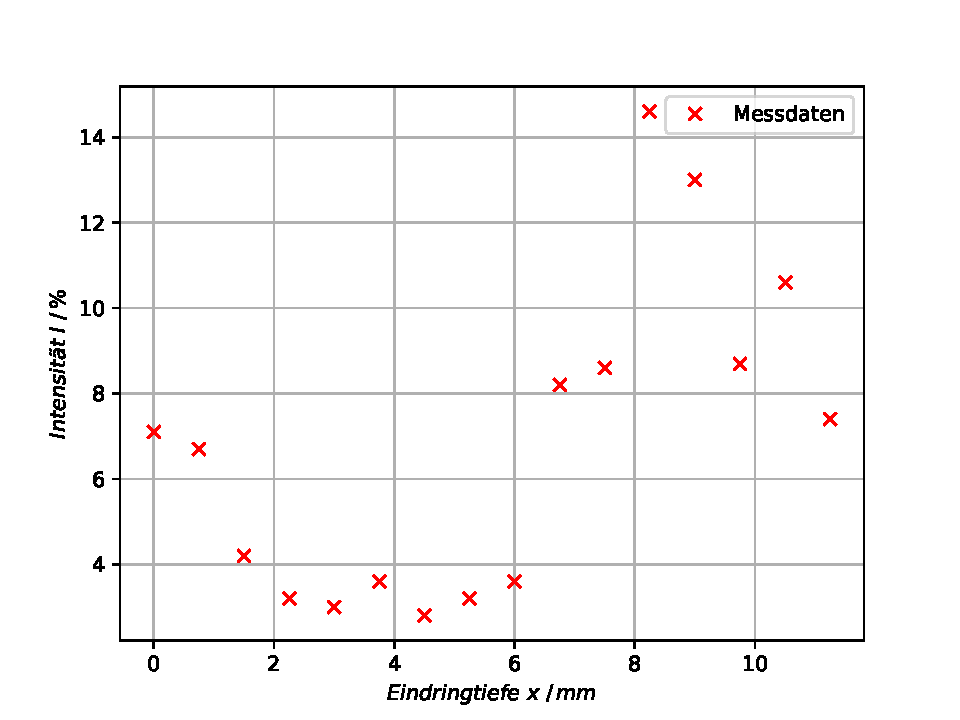
\includegraphics[width=0.8\linewidth]{streu_48.pdf}
	\caption{Streuintensität $I$ als Funktion der Eindringtiefe $x$ bei $\dot{V} = 4{,}8\,\symup{\frac{l}{min}}$.}
	\label{fig:profil2}
\end{figure}


\begin{figure}[h!tbp]
	\centering
	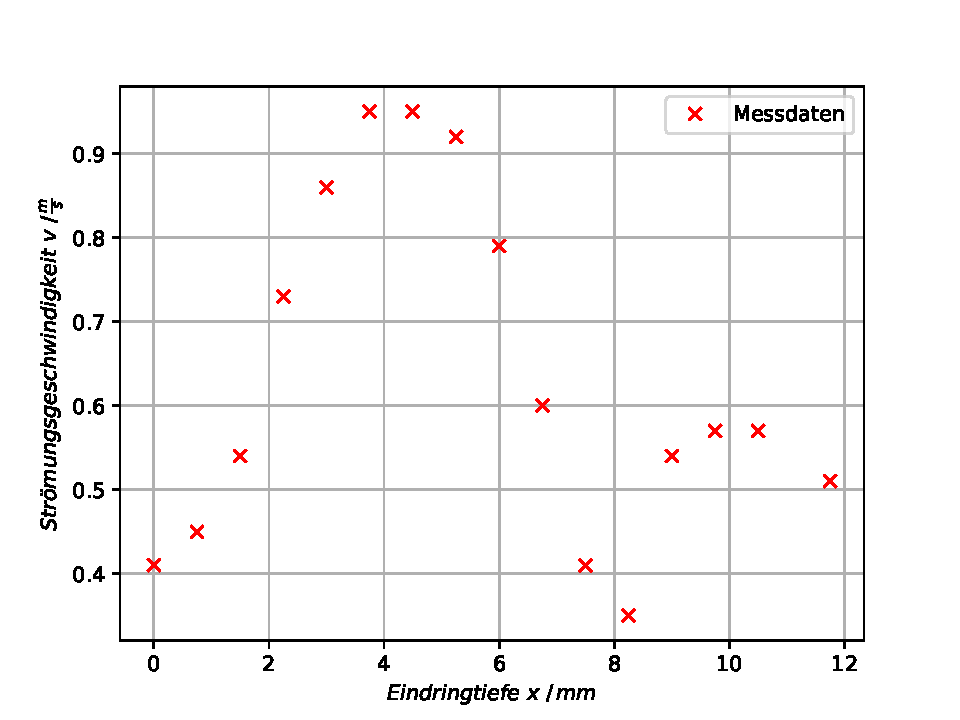
\includegraphics[width=0.8\linewidth]{geschw_34.pdf}
	\caption{Strömungsgeschwindigkeit $v$ als Funktion der Eindringtiefe $x$ bei $\dot{V} = 3{,}4\,\symup{\frac{l}{min}}$.}
	\label{fig:profil3}
\end{figure}


\begin{figure}[h!tbp]
	\centering
	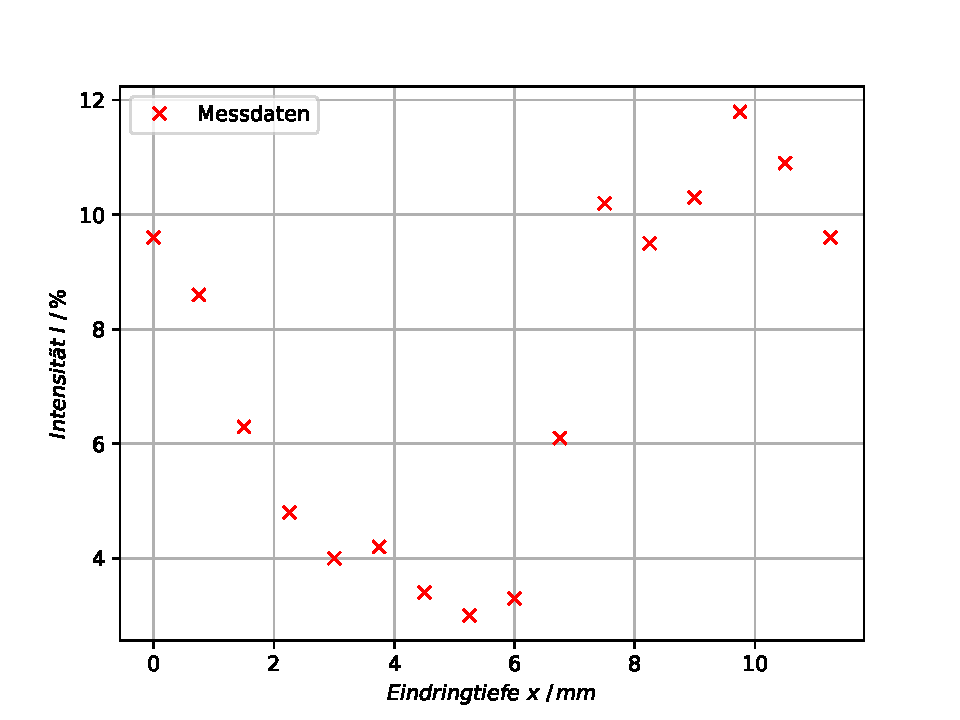
\includegraphics[width=0.8\linewidth]{streu_34.pdf}
	\caption{Streuintensität $I$ als Funktion der Eindringtiefe $x$ bei $\dot{V} = 3{,}4\,\symup{\frac{l}{min}}$.}
	\label{fig:profil4}
\end{figure}
